\begin{figure}
    \begin{center}
    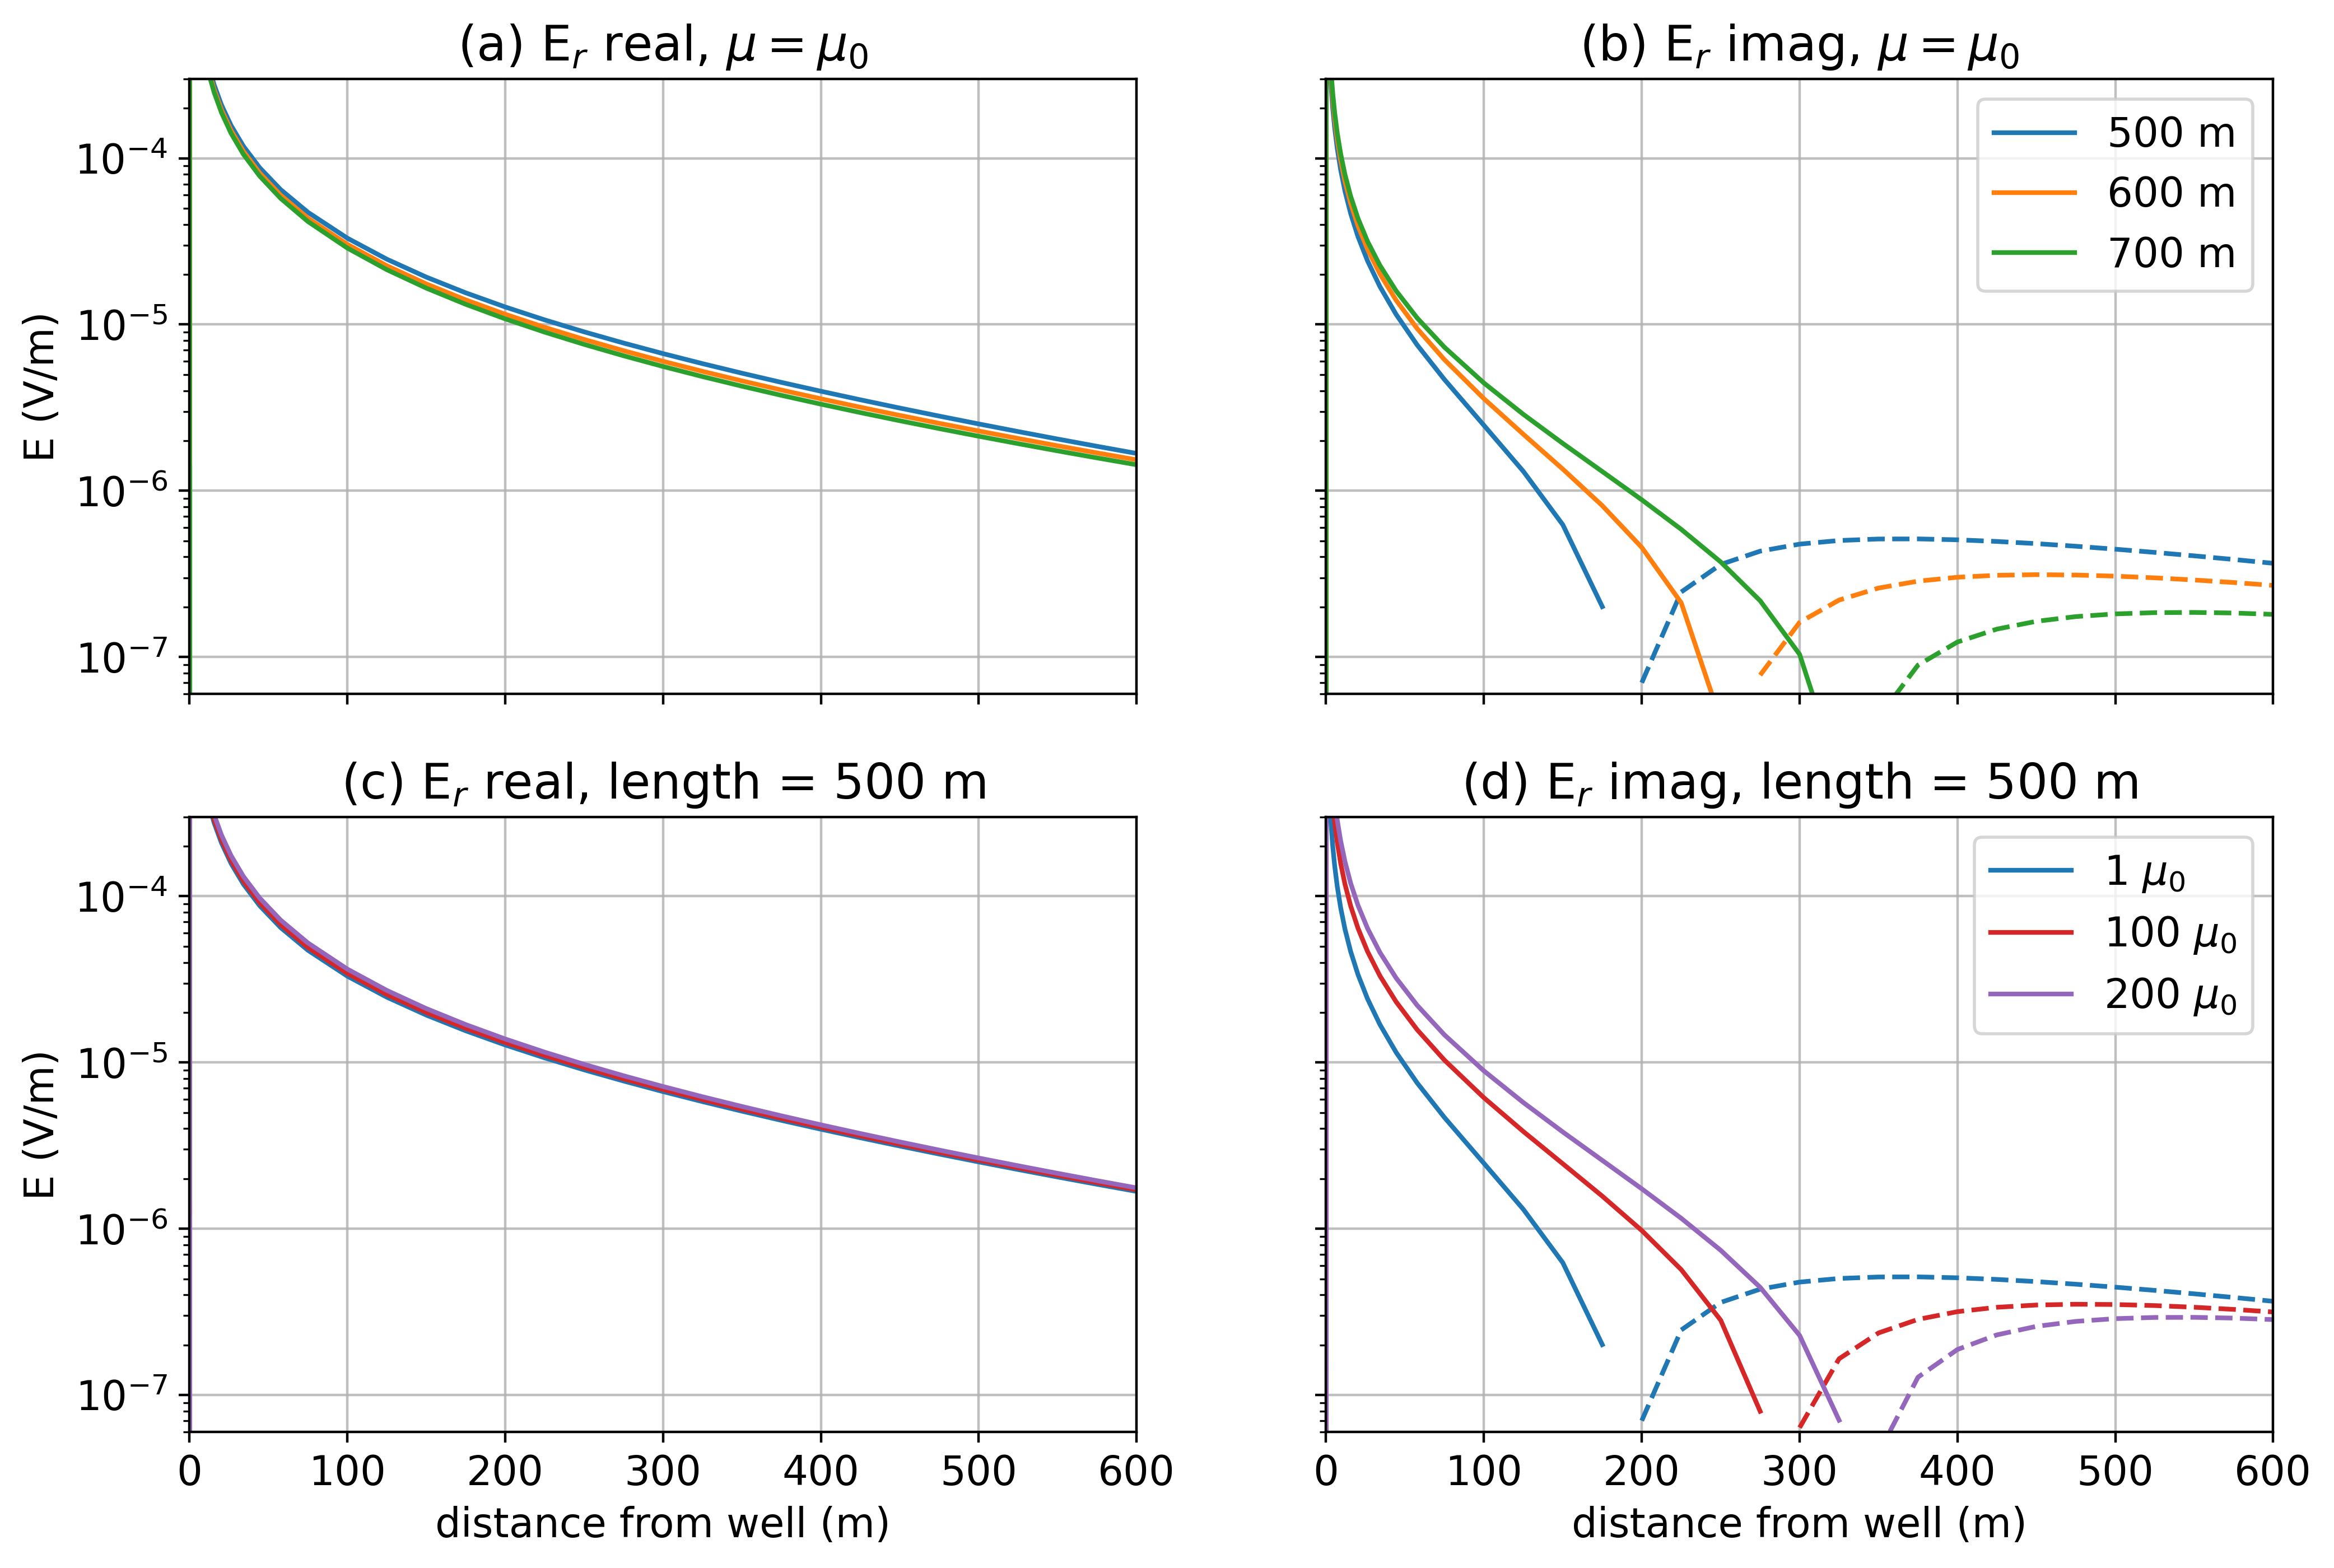
\includegraphics[width=\textwidth]{figures/motivation-casing-integrity-500.png}
    \end{center}
\caption{
    Radial electric field data for a top-casing experiment at 5 Hz. The top row shows the (a) real and (b) imaginary components for different lengths of a conductive well ($\sigma=5\times10^6$ S/m, $\mu=\mu_0$) in a 10$\Omega$m background. The bottom row shows the (c) real and (d) imaginary components for a 500m long well as the permeability is varied. The outer diameter of the casing is 10cm, and it is 2cm thick. The return electrode is 500m from the casing, and the receivers are along a line $180^\circ$ from the transmitter wire.
}
\label{fig:motivation-casing-integrity}
\end{figure}



